\section{Model Calibration}\label{app.model.cal}
Table~\ref{tab:par.defs} gives the short names (used in code and some results figures),
definitions, and distributions (prior and posterior mean and 95\%~CI)
of the calibrated model parameters ($N = 73$).
The exact sampling distributions, constraints, and application of each parameter to define
the complete set of model inputs is available online:\\
\hreftt{github.com/mishra-lab/hiv-fsw-art/blob/master/code/model/params.py}
% \begin{longtable}{crl}
  {\label{tab:par.defs}Definitions of calibrated parameters}
  {* & Parameter & Definition}{%
    * relational sampling constraints (see \sref{app.model.cal.constr});
    FSW: female sex worker;
    p12m: past 12 months;
    $\beta$: per-act probability of HIV transmission;
    GUD: any genital ulcer disease in p12m;
    ART: antiretroviral therapy;
    VLS: viral load suppression;
    additional relative (aR): relative value beyond one, \eg $R = 1.5 \rightarrow aR = 0.5$;
    prevalence interpolator (iP): \eg $P_0 = 0.2, P_1 = 0.4, iP_x = 0.5 \rightarrow P_x = 0.3$;
    all rates in per-year;
    all durations in years;
    all parameters reflect stratum averages.}
  \csvreader[head to column names]{model/app/par.defs.csv}{}
    {\small\constr & \texttt{\parameter} & \footnotesize\definition\\}
\end{longtable}
 (*) moved below for landscape pagebreak
%===================================================================================================
\subsection{Relational Sampling Constraints}\label{app.model.cal.constr}
Several relational constraints were imposed on calibrated parameter values during sampling.
Incorporating constraints within Latin hypercube sampling is challenging \cite{Petelet2010}.
Thus, for each set of constraints below, the selected parameters
were sampled randomly (not via Latin hypercube) and repeated until all constraints were satisfied;
as noted in \sref{app.math.distr.jsam},
this sampling strategy effectively changes the prior distribution
to reflect both the original prior and the specified constraints.
\begin{itemize}\singlespacing
  \item[a.] \texttt{K_swo_fsw_l * RC_swo_fsw_h:l * F_swo + K_swr_fsw_l * RC_swr_fsw_h:l * F_swr < 2*365}\\
            where: \texttt{K_swx_fsw_l = C1m_swx_fsw_l * dur_swx / (dur_swx + 1/12)}
  \item[b.] Let ``\texttt{c_}'' denote \texttt{PF_condom_}:\\
            \texttt{c_msp_2006 < c_msp_2016}\\
            \texttt{c_cas_2006 < c_cas_2016}\\
            \texttt{c_swo_2002 < c_swo_2011 < c_swo_2014}\\
            \texttt{c_swr_2002 < c_swr_2011 < c_swr_2014}\\
            \texttt{c_msp_2006 < c_cas_2006}\\
            \texttt{c_msp_2016 < c_cas_2016}\\
            \texttt{c_swr_2002 < c_swo_2002}\\
            \texttt{c_swr_2011 < c_swo_2011}\\
            \texttt{c_swr_2014 < c_swo_2014}
  \item[c.] \texttt{1 <= (Rbeta_acute * dur_acute) <= 63}
  \item[d.] \texttt{P_gud_fsw_l > .07}\\
            \texttt{(P_gud_fsw_l * RP_gud_fsw_h:l) < 1}
\end{itemize}
\begin{longtable}{crl}
  {\label{tab:par.defs}Definitions of calibrated parameters}
  {* & Parameter & Definition}{%
    * relational sampling constraints (see \sref{app.model.cal.constr});
    FSW: female sex worker;
    p12m: past 12 months;
    $\beta$: per-act probability of HIV transmission;
    GUD: any genital ulcer disease in p12m;
    ART: antiretroviral therapy;
    VLS: viral load suppression;
    additional relative (aR): relative value beyond one, \eg $R = 1.5 \rightarrow aR = 0.5$;
    prevalence interpolator (iP): \eg $P_0 = 0.2, P_1 = 0.4, iP_x = 0.5 \rightarrow P_x = 0.3$;
    all rates in per-year;
    all durations in years;
    all parameters reflect stratum averages.}
  \csvreader[head to column names]{model/app/par.defs.csv}{}
    {\small\constr & \texttt{\parameter} & \footnotesize\definition\\}
\end{longtable}
 % (*)
%===================================================================================================
\subsection{Results}\label{app.model.cal.res}
This section provides additional results to supplement \sref{model.res.cal}.
\begin{figure}[h]
  \centering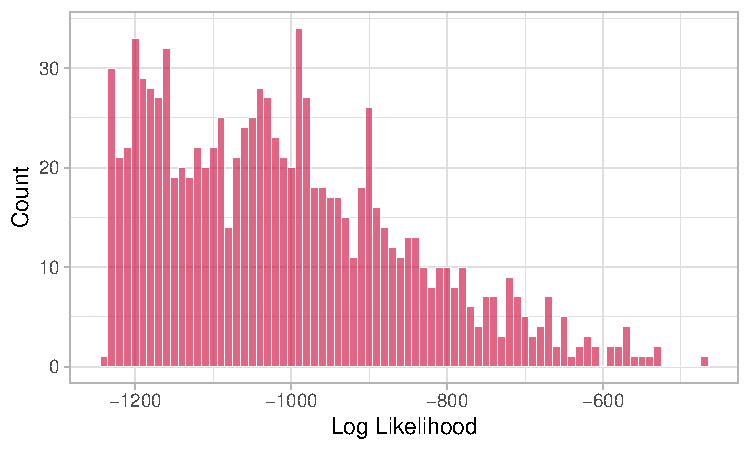
\includegraphics[width=.7\linewidth]{fit.ll.base.pdf}
  \caption{Distribution of log-likelihoods among model fits}
  \label{fig:fit.ll}
  \floatfoot{\fffit.}
\end{figure}
\par
Figures~\ref{fig:fit.prevalence1v2}~and~\ref{fig:fit.incidence1v2}
illustrate the modelled ratios of HIV prevalence and incidence, respectively,
between selected risk groups, and associated calibration targets.
Figure~\ref{fig:fit.pop} similarly illustrates the total Eswatini population size aged 15--49, and
Figure~\ref{fig:fit.condom} illustrates condom use within each partnership type.
\begin{figure}[h]
  \centering\includegraphics[scale=.5]{fit.prevalence1v2.base.all.pdf}
  \caption{Modelled HIV prevalence ratios between selected risk groups
    and associated calibration targets}
  \label{fig:fit.prevalence1v2}
  \floatfoot{\fffit; \ffribbon; \ffpbar.}
\end{figure}
\begin{figure}[h]
  \centering\includegraphics[scale=.5]{fit.incidence1v2.base.all.pdf}
  \caption{Modelled HIV incidence ratios between selected risk groups
    and associated calibration targets}
  \label{fig:fit.incidence1v2}
  \floatfoot{\fffit; \ffribbon; \ffpbar.}
\end{figure}
\begin{figure}[h]
  \begin{minipage}[t]{.54\linewidth}
    \centering\includegraphics[scale=.5]{fit.prevalence.anc.pdf}
    \caption{HIV prevalence data from antenatal care clinics in Eswatini}
    \label{fig:fit.prevalence.anc}
  \end{minipage}\hfill
  \begin{minipage}[t]{.44\linewidth}
    \centering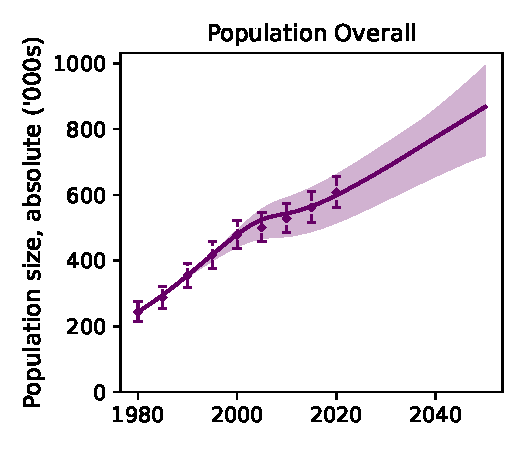
\includegraphics[scale=.5]{fit.NX.base.all.pdf}
    \caption{Modelled Eswatini population aged 15--49
    and associated calibration targets}
    \label{fig:fit.pop}
  \end{minipage}
  \floatfoot{\fffit; \ffribbon; \ffpbar.}
\end{figure}
\begin{figure}[h]
  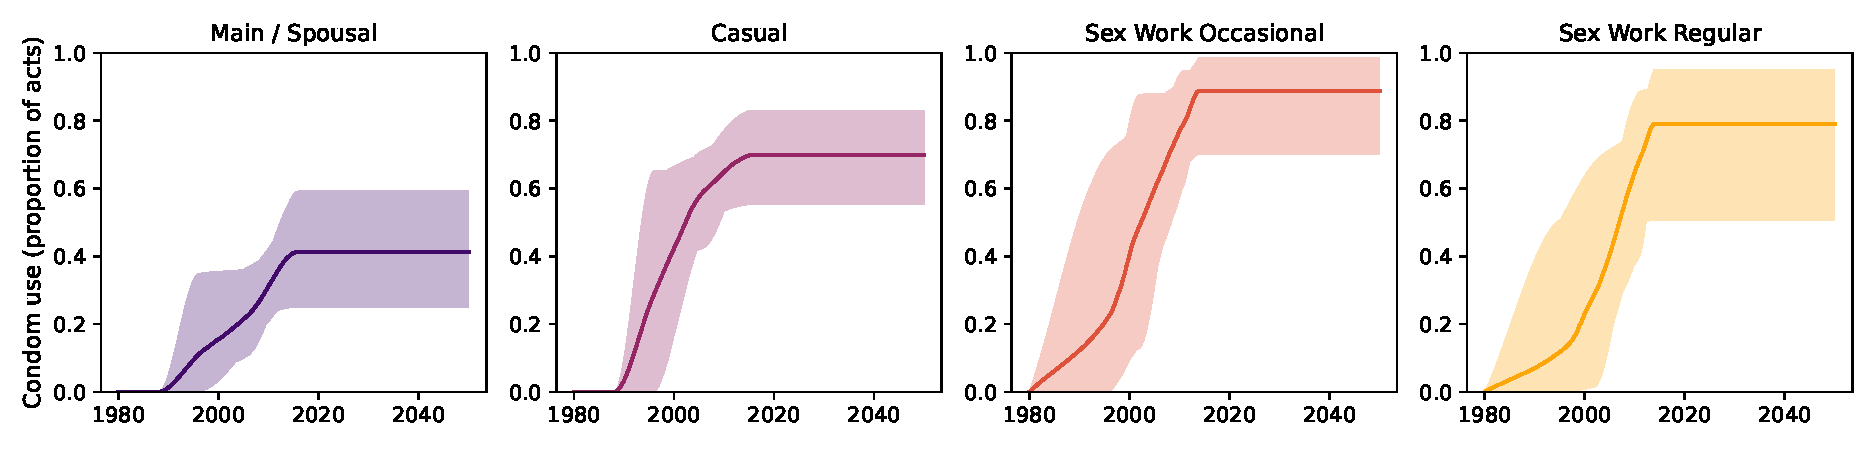
\includegraphics[scale=.5]{fit.condom.base.all.pdf}
  \caption{Modelled condom use within different partnership types}
  \label{fig:fit.condom}
  \floatfoot{\fffit; \ffribbon.}
\end{figure}
